\documentclass{article}
% 导入导言区
% 该文件仅负责格式配置或通用命令
% 只适用于该论文的自定义命令放到 预定义.tex
% 中文
\usepackage{ctex}
% 浮动体控制
\usepackage{float}
% 页面
\usepackage[left=2cm,right=2cm,top=2.5cm,bottom=2cm]{geometry}
% 解决字体警告
\usepackage{anyfontsize}
% 设置英文字体
\setmainfont{Times New Roman}
% 图片宏包
\usepackage{graphicx}
% 图片文件夹路径
\graphicspath{{../Output/}}
% 文献引用风格
\usepackage{natbib}
% 规定论文格式
\usepackage[number]{gbt7714}
% 颜色
\usepackage{xcolor}
% 字体
\usepackage{fontspec}
% 间距控制
\usepackage{setspace}
% 子图
\usepackage{subfigure}
% 页眉页脚
\usepackage{fancyhdr}
\pagestyle{fancy}
\fancyhf{}
\fancyhead[C]{\songti\zihao{5}河北农业大学学士学位论文}
\fancyfoot[C]{\thepage}
% 数学相关宏包
\usepackage{amsthm,amsmath,amssymb,mathrsfs}
% 图表公式章节编号
\renewcommand{\thetable}{\thesection-\arabic{table}}
\renewcommand{\thefigure}{\thesection-\arabic{figure}}
\renewcommand{\theequation}{\thesection.\arabic{equation}}
\makeatletter
\@addtoreset{table}{section}
\@addtoreset{figure}{section}
\@addtoreset{equation}{section}
\makeatother
% 超链接
\usepackage[
    colorlinks,
    linkcolor=black,
    anchorcolor=black,
    citecolor=black
]{hyperref}
% 流程图
\usepackage{tikz}
\usetikzlibrary{shapes.geometric,arrows}
\tikzstyle{startstop} = [rectangle,rounded corners, minimum width=1cm,minimum height=1cm,text centered, draw=black,fill=red!30]
\tikzstyle{io} = [trapezium, trapezium left angle = 70,trapezium right angle=110,minimum width=1cm,minimum height=1cm,text centered,draw=black,fill=blue!30]
\tikzstyle{process} = [rectangle,minimum width=1cm,minimum height=1cm,text centered,text width =3cm,draw=black,fill=orange!30]
\tikzstyle{decision} = [diamond,minimum width=1cm,minimum height=1cm,text centered,draw=black,fill=green!30]
\tikzstyle{arrow} = [thick,->,>=stealth]
% 英文摘要
\newenvironment{enabstract}{
    \par\small
    \noindent\mbox{}\hfill{\bfseries \zihao{-3} ABSTRACT}\hfill\mbox{}\par
    \vskip 2.5ex}{\par\vskip 2.5ex}
% 中文摘要
\newenvironment{cnabstract}{
    \par\small
    \noindent\mbox{}\hfill{\bfseries \heiti\zihao{-3} 摘  要}\hfill\mbox{}\par
    \vskip 2.5ex}{\par\vskip 2.5ex}
% 代码环境
\usepackage{listings}
% 代码格式设置
\lstset{
    % 语言
    language=python,
    % 自动换行
    breaklines=true,
    % 行号
    numbers=left,
    % 字符串显示空格
    showstringspaces=false,
    % 基础字体设置
    basicstyle=\small\fontspec{Monaco},
    % 字符串风格
    stringstyle=\color{purple},
    % 注释风格
    commentstyle=\color{gray},
    % 关键字风格
    keywordstyle=\color{blue},
    % 左侧margin
    xleftmargin = 25pt,
    % 添加frame
    frame = tb,
    % 设置frame左侧margin
    framexleftmargin = 20pt,
}
% 导入预定义指令
% 该文件仅负责只适用于该论文的自定义命令
% 格式配置或通用指令放到 导言区.tex
% 积分算子
\newcommand{\dt}[1]{\frac{\mathrm{d}#1}{\mathrm{d}t}}
% 概率
\renewcommand{\P}[2]{P^{#1}_{#2}}
% 人群
\newcommand{\T}[2]{T^{#1}_{#2}}
% 感染机制
\newcommand{\TP}[3]{\T{#1}{#2}&=\P{#1}{#2}#3}
% 概率文本
\newcommand{\PText}[2]{$#1$群体转变为$#2$群体的概率}
% 全局有效再生数
\def\rot{1.588}
% 基本再生数
\def\ro{6.62}
% 有效再生数
\def\rt{1.573}
% 图片宽度
\def\imagewidth{0.65\textwidth}
\def\smallimagewidth{0.45\textwidth}
% 显示数据表格
\newcommand{\showdatatable}[1]{
    \input{Table/#1模型拟合数据.tex}
}
% 显示隔离前后数据表格
\newcommand{\showdatatables}[1]{
    \input{Table/#1隔离前模型拟合数据.tex}
    \input{Table/#1隔离后模型拟合数据.tex}
}
% 显示表格
\newcommand{\showtable}[1]{
    \begin{table}[H]
        \centering
        \caption{#1模型拟合参数\label{table:#1模型拟合参数}}
        \input{Table/#1.tex}
    \end{table}
}
% 显示隔离后表格
\newcommand{\showtables}[1]{
    \begin{table}[H]
        \centering
        \caption{#1模型隔离前后拟合参数\label{table:#1模型隔离前后拟合参数}}
        \input{Table/#1隔离.tex}
    \end{table}
}
% 显示图片
\newcommand{\showfigure}[1]{
    \begin{figure}[H]
        \centering
        \includegraphics[width=\imagewidth]{#1.png}
        \caption{#1模型拟合图像\label{figure:#1模型拟合图像}}
    \end{figure}
}
% 显示隔离后图片
\newcommand{\showfigures}[1]{
    \begin{figure}[H]
        \centering
        \subfigure[#1模型隔离前拟合图像]{
            \includegraphics[width=\smallimagewidth]{#1隔离前.png}
        }
        \subfigure[#1模型隔离后拟合图像]{
            \includegraphics[width=\smallimagewidth]{#1隔离后.png}
        }
        \caption{#1模型隔离前后拟合图像\label{figure:#1模型隔离前后拟合图像}}
    \end{figure}
}
% SIR模型
\def\SIR{
    \begin{table}[H]
        \centering
        \caption{SIR模型参数表}
        \begin{tabular}{ll}
            \hline
            符号     & 含义         \\
            \hline
            $\alpha$ & \PText{S}{I} \\
            $\beta$  & \PText{I}{R} \\
            \hline
        \end{tabular}
    \end{table}
    \def\SI{IS\alpha}
    \def\IR{I\beta}
    \begin{align}
        \dt{S} & = -\SI      \\
        \dt{I} & = \SI - \IR \\
        \dt{R} & = \IR
    \end{align}
}
\def\SEIR{
    \begin{table}[H]
        \centering
        \caption{SEIR模型参数表}
        \begin{tabular}{ll}
            \hline
            符号       & 含义         \\
            \hline
            $\alpha$   & \PText{S}{E} \\
            $\gamma$   & \PText{E}{I} \\
            $\epsilon$ & \PText{E}{R} \\
            $\beta$    & \PText{I}{R} \\
            \hline
        \end{tabular}
    \end{table}
    \def\SE{(I+E)S\alpha}
    \def\EI{E\gamma}
    \def\ER{E\epsilon}
    \def\IR{I\beta}
    \begin{align}
        \dt{S} & = -\SE            \\
        \dt{E} & = \SE - \EI - \ER \\
        \dt{I} & = \EI - \IR       \\
        \dt{R} & = \IR +\ER
    \end{align}
}
\def\SEIRD{
    \begin{table}[H]
        \centering
        \caption{SEIRD模型参数表}
        \begin{tabular}{ll}
            \hline
            符号       & 含义         \\
            \hline
            $\alpha$   & \PText{S}{E} \\
            $\gamma$   & \PText{E}{I} \\
            $\epsilon$ & \PText{E}{R} \\
            $\beta$    & \PText{I}{R} \\
            $\delta$   & \PText{I}{D} \\
            \hline
        \end{tabular}
    \end{table}
    \def\SE{(I+E)S\alpha}
    \def\EI{E\gamma}
    \def\ER{E\epsilon}
    \def\IR{I\beta}
    \def\ID{I\delta}
    \begin{align}
        \dt{S} & = -\SE            \\
        \dt{E} & = \SE - \EI - \ER \\
        \dt{I} & = \EI - \IR - \ID \\
        \dt{R} & = \IR + \ER       \\
        \dt{D} & = \ID
    \end{align}
}
\def\SEIRS{
    \begin{table}[H]
        \centering
        \caption{SEIRS模型参数表}
        \begin{tabular}{ll}
            \hline
            符号       & 含义         \\
            \hline
            $\alpha$   & \PText{S}{E} \\
            $\gamma$   & \PText{E}{I} \\
            $\epsilon$ & \PText{E}{R} \\
            $\beta$    & \PText{I}{R} \\
            $\delta$   & \PText{I}{D} \\
            $\theta$   & \PText{R}{I} \\
            \hline
        \end{tabular}
    \end{table}
    \def\SE{(I+E)S\alpha}
    \def\EI{E\gamma}
    \def\ER{E\epsilon}
    \def\IR{I\beta}
    \def\ID{I\delta}
    \def\RI{R\theta}
    \begin{align}
        \dt{S} & = -\SE                  \\
        \dt{E} & = \SE - \EI - \ER       \\
        \dt{I} & = \RI + \EI - \IR - \ID \\
        \dt{R} & = \IR - \RI + \ER       \\
        \dt{D} & = \ID
    \end{align}
}
\title{\heiti \zihao{-2} 基于SEIR的病毒传播模型}
\author{\songti \zihao{-4} 信息与计算科学 1601 骆天奇\\指导教师\ 王斌}
\date{}
\begin{document}
\begin{titlepage}
      \begin{center}
    \vspace{2cm}
    \begin{spacing}{2.0}
        \textbf{\zihao{1}河北农业大学本科毕业论文}
    \end{spacing}
    \vfill
    \zihao{3}
    \songti
    \begin{tabular}[b]{cc}
        \rule{0pt}{1cm}\textbf{学  院:} & 理学院             \\\cline{2-2}
        \rule{0pt}{1cm}\textbf{学生姓名:} & 骆天奇             \\\cline{2-2}
        \rule{0pt}{1cm}\textbf{学  号:} & 2016254060407      \\\cline{2-2}
        \rule{0pt}{1cm}\textbf{专业班级:} & 信息与计算科学1601 \\\cline{2-2}
        \rule{0pt}{1cm}\textbf{教师姓名:} & 王斌               \\\cline{2-2}
        \rule{0pt}{1cm}\textbf{职  称:} & 讲师               \\\cline{2-2}
    \end{tabular}
    \\
    \vspace{3cm}
    \textbf{二零二零 年 五 月 二十 日}
\end{center}
\clearpage
      \maketitle
      % 摘要
\begin{cnabstract}
	\songti \zihao{-4}
	\absemph{目的:}
	建立一系列流体动力学模型,
	拟合新型冠状病毒肺炎的疫情的官方发布数据,
	在其中找出一个最为有效的预测模型,
	为今后与之类似的疫情防控提供一种预测方法。
	\absemph{方法:}
	基于SIR预测模型,
	根据病毒特点一步步迭代构建新的预测模型。
	并基于官方公布的数据进行拟合,
	根据拟合效果选择最优模型,
	从使用最优模型的最佳估计参数中提取有效信息。
	\absemph{结果:}
	在提出的三个模型($SIR$、$SEIRD$、$SEIRS$)中,
	$SEIRD$模型最符合疫情传播趋势,
	通过分析$SEIRD$模型的最优估计参数,
	得出了疫情的初期(未隔离甚至人口密集状态下)$R_0=5.5937$,
	疫情后期(隔离措施到位)$R_0=1.242$,
	整个疫情周期$R_0=1.764$,
	基本符合官方发布数据及众多文献的结论。
	说明该模型可以较为准确的描述疫情传播过程,
	可用于类似传染病的预测。
	\\
	\absemph{关键字:} SEIR, 数学模型,传染病, COVID-19
\end{cnabstract}
\begin{enabstract}
	\zihao{-4}
	\absemph{Target:}
	Establish a series of fluid dynamic models to fit the official release data of the new coronavirus pneumonia epidemic,
	find one of the most effective prediction models,
	and provide a prediction method for similar epidemic prevention and control in the future.
	\absemph{Method:}
	Based on the SIR prediction model,
	iteratively builds a new prediction model step by step according to the characteristics of the virus.
	Based on the officially published data,
	the optimal model is selected according to the fitting effect,
	and effective information is extracted from the best estimated parameters using the optimal model.
	\absemph{Result:}
	Among the three models proposed ($SIR$, $SEIRD$, $SEIRS$),
	the $SEIRD$ model is most in line with the epidemic propagation trend.
	By analyzing the optimal estimation parameters of the $SEIRD$ model,
	the initial stage of the epidemic (unisolated or even densely populated) is obtained $R_0 = 5.5937$,
	late in the epidemic (isolation measures in place) $R_0 = 1.242$,
	the entire epidemic cycle $R_0 = 1.764$,
	basically in line with the official data and the conclusions of many literature.
	It shows that the model can describe the spreading process of epidemic situation more accurately and can be used to predict similar infectious diseases.
	\\
	\absemph{Key Words:} SEIR, mathematical model, epidemic, COVID-19
\end{enabstract}
      % 不显示页码
      \thispagestyle{empty}
      \clearpage
      \tableofcontents
      % 不显示页码
      \thispagestyle{empty}
\end{titlepage}
\songti \zihao{-4}
\section{引言}
\subsection{研究背景}
新型冠状病毒疫情发生以来,
引起全世界众多媒体和专家学者的关注。
各有关部门和地方在
疫情防控、患者救治、科研攻关、物资保障
等方面采取了一系列措施。
传染病的扩散对人们的健康和生命安全造成了巨大威胁,
同时严重影响了社会生活和国民经济。
人们渴望知道何时将完全控制该传染病
以及人们的工作和生活将何时步入正规。
预测疫情的趋势可以提前做好医疗资源的配备,
有序进行复工复产的安排并坚定人们战胜疫情的信心,
因此构建一个该类病毒的预测模型是有价值的。
\subsection{研究目的}
新型冠状病毒(COVID-19)的爆发引起了国内外众多关注,
预测传染病的传布趋势可以大致得知疫情蔓延趋势及结束时间以提前做出安排。
本文希望通过构建$SIR$模型及其多个衍生模型,
结合COVID-19的疫情数据进行拟合分析,
探究传染病的传播规律并预测其发展趋势。
在尝试的几种模型中找寻适合用于此类病毒的模型。
\section{研究基础}
\subsection{文献综述}
\citeauthor{对流行病数学理论的贡献}在\citeyear{对流行病数学理论的贡献}年针对传染病问题提出了$Compartmental$模型\cite{对流行病数学理论的贡献},将人群划分为多个部分,并假设同一部分中的每个人都具有相同的特征从而建立积分方程推导传染病的传播过程;
\citeauthor{Kermack-McKendrick确定性流行病模型的推广}于\citeyear{Kermack-McKendrick确定性流行病模型的推广}年对$Compartmental$模型做出了推广,将人群为易感染者$S$,感染者$I$,康复者$R$,提出了经典的$SIR$模型\cite{Kermack-McKendrick确定性流行病模型的推广},后来的$SEIR$,$SEIS$,$MSEIR$等众多模型都是以$SIR$模型为基础衍生出来的;
王小莉等人于\citeyear{应用SEIR模型预测2009年甲型H1N1流感流行趋势}年根据不同因素下(年龄、地区、生活习惯等)的数据建立$SEIR$模型,探究预测甲型H1N1流感在不同因素下的传播情况\cite{应用SEIR模型预测2009年甲型H1N1流感流行趋势};
杨旭颖等人于\citeyear{基于SEIR的社交网络信息传播模型}年将$SEIR$模型用于模拟社交网络的信息传播机制\cite{基于SEIR的社交网络信息传播模型},目的是预测社交网络上的信息传播趋势;
王晓红于\citeyear{一类具有潜伏期的SEIR手足口病模型的研究}年将$SEIR$模型用于预测手足口病的疫情趋势\cite{一类具有潜伏期的SEIR手足口病模型的研究},并考虑了康复者复发的情况(即后来的$SEIRS$模型),得到了足口病的基本再生数并对模型进行了动力学分析:平衡点的存在性和稳定性;
崔金栋等人于\citeyear{基于改良SEIR模型的微博话题式信息传播研究}年以微博信息传播中的SEIR模型为出发点,综合考虑微博网络中话题式信息的衍生特性,构建改良式的微博话题式信息传播H-SEIR模型\cite{基于改良SEIR模型的微博话题式信息传播研究},并运用MATLAB进行模拟仿真,对微博中话题式信息传播影响因素和对应的控制策略进行研究;
赵世磊等人通过$SUQC$模型\cite{通过流行病学建模表征传播和确定COVID-19的控制策略}(在$SEIR$模型基础上加入潜伏期感染和隔离条件)基于官方每日发布的数据不断调整隔离参数及传染率,最终得出疫情在不同阶段的隔离率,确诊率及病毒生殖率(即传播率)并对疫情最终影响人数做出预测,其模型较为单一,结果可能不够准确,但将参数分段考虑的方式值得借鉴;
李静华运用五种不同的方法\cite{估计2019年新型冠状病毒的流行性:数学建模研究}(分别是指数增长,最大似然法,顺序贝叶斯方法,时间序列分析,$SEIR$模型)对病毒在2月8日前后及整个疫情期间的传播率做出了估计,结论较为可靠,但并没有进一步预测未来的疫情趋势;
周慧娟等人通过$SEIQ$模型\cite{中国COVID-19爆发的流行动力学模型和控制}(在$SEIR$模型基础上加入隔离人群$Q$)通过$Montecarlo$方法模拟了两个独立的泊松过程(分别是每日暴露病例和个体潜伏时间)讨论在不同环境的不同隔离措施下病毒的感染率;
金华潘等人通过对$SEIR$模型做出一系列改动\cite{2019年冠状病毒疾病控制策略的有效性:SEIR动态建模研究}(其中包括超级传染,治疗等)计算了2月16日之前的病毒基础生殖率,但该模型并未考虑隔离情况,因此预测可能有较大偏差,但其对治疗人群的引入值得借鉴;
\citeauthor{估计2020年公主邮轮船上2019年新型冠状病毒的无症状比率}使用哈密顿蒙特卡洛($HMC$)的贝叶斯框架\cite{估计2020年公主邮轮船上2019年新型冠状病毒的无症状比率}预测封闭的小范围环境(游轮环境)的未感染人数,可以用来粗略估计封闭的大范围环境(封闭下的城市)的未感染人数;
战军湛等人基于$SEIR$模型借助人口迁移学通过城市间人口流动数据\cite{结合人类迁移数据的2019年冠状病毒疾病在中国传播的建模与预测}预测疫情在城市间的传播,但没有考虑隔离的情况并轻视了疫情期间人口流动严重停滞的情况,故其预测结果偏差较大,不可用于预测结果参考,但其以城市为基本单元的思考方式值得借鉴;
彭鹏等人基于广义动力学模型\cite{基于动力学模型的中国COVID-19流行病学分析}引入七个状态(在原有的四个状态基础上新加入隔离,死亡,免疫)结合官方发布数据,预测疫情进展并对疫情持续时间做出估计,可用于结果评测;
张良禄等人通过基础$SEIR$建模\cite{SEIR建模分析与新型冠状病毒的斗争何时在武汉结束},将1月22日到2月12日间的数据以2月7日为界限分别建立了模型,得出一系列基础参数并给出了预测结果,但其对疫情过于乐观,并未考虑隔离及潜伏期可传染,不适用于长期预测;
\citeauthor{协调基本生殖数量及其不确定性的早期暴发估计:新型冠状病毒(SARS-CoV-2)暴发的框架和应用}认为单纯的将病毒生殖数看作一个常量已不适用于COVID-19,故将病毒基本生殖数划分为三个关键量\cite{协调基本生殖数量及其不确定性的早期暴发估计:新型冠状病毒(SARS-CoV-2)暴发的框架和应用}(指数增长率,平均生成间隔,生成间隔离散度)并结合官方数据来估算病毒的传染率,其思想及结果值得借鉴,或许将一些参数(如:传染率,治愈率)设计为一个与时间有关的分段函数(以隔离措施及医学进展的时间点为断点)比较合适。
\subsection{概念解释}
\subsection{理论基础}
\citeauthor{对流行病数学理论的贡献}在\citeyear{对流行病数学理论的贡献}年研究黑死病时提出了仓室模型,模型中将人口分为三类:
\begin{itemize}
    \item 易感者(susceptibles),$S$人群
    \item 感染者(infectives),$I$人群
    \item 康复者(recovered),$R$人群
\end{itemize}
\par 将其称为$SIR$
\cite{对流行病数学理论的贡献}模型。
\citeauthor{Kermack-McKendrick确定性流行病模型的推广}在\citeyear{Kermack-McKendrick确定性流行病模型的推广}年对其进行了推广\cite{Kermack-McKendrick确定性流行病模型的推广},证明其广泛的适用性。
\par $SIR$模型的建立基于几个假设\cite{对流行病数学理论的贡献}:
\begin{itemize}
    \item 人口总数保持常量(包含死亡人数)
    \item 单位时间$t$传染人数与$S$和$I$人数成正比,即$S\to I = \alpha SI$
    \item 单位时间$t$康复人数与$I$成正比,即$I\to R = \beta I$
\end{itemize}
\begin{table}[H]
    \centering
    \caption{SIR模型符号表}
    \label{table:SIR模型符号表}
    \begin{tabular}{ll}
        \hline
        符号     & 含义         \\
        \hline
        S        & 易感者       \\
        I        & 感染者       \\
        R        & 康复者       \\
        $\alpha$ & \PText{S}{I} \\
        $\beta$  & \PText{I}{R} \\
        \hline
    \end{tabular}
\end{table}
\par 感染机制如下:
\begin{align}
    S(t) & \xrightarrow \alpha I(t) \\
    I(t) & \xrightarrow \beta R(t)
\end{align}
\par 可以用积分方程表示为
\begin{align}
    \dt{S} & = -\alpha SI          \\
    \dt{I} & = \alpha SI - \beta I \\
    \dt{R} & = \beta I
\end{align}
\subsection{使用工具}
使用python实现爬虫获取数据(见附录\ref{appendix:数据})、
使用scipy库进行积分求解及数据拟合(见\ref{section:数据拟合与分析})、
使用pyecharts库绘制图像。
\section{模型研究}
\subsection{模型解释}
\par 通过微分方程来描述美观简练,
但在扩建模型时会有一些麻烦:
由表\ref{table:SIR模型符号表}可预见,
随着划分人群的增多,
人群间感染机制也随之复杂,
不同人群之间转变率的符号也会增多或者改变含义,
这会使读者对符号的理解产生负面的路径依赖影响,
对于模型的扩建是十分不利的。
\par $SIR$模型的本质为人群间的转移,
只要理解人群间的转移方程便可了解模型的结构。
而这类模型都是在总人数固定的前提下进行的,
所以通过状态转移方程即可得出微分方程,
传染病问题中,
状态转移等价于感染机制,
为了更为清晰的描述人群间的感染机制,
本文将引入新的描述方式。
\begin{table}[H]
    \centering
    \caption{另一种模型符号表示}
    \begin{tabular}{ll}
        \hline
        符号       & 含义                              \\
        \hline
        $\P{a}{b}$ & a群体变为b群体的概率              \\
        $\T{a}{b}$ & 单位时间$t$内a群体变为b群体的人数 \\
        \hline
    \end{tabular}
\end{table}
\par 将a到b群体的转换概率用$\P{a}{b}$表示,单位时间内a到b群体转变的人数为$\T{a}{b}$。
\par 感染机制如下:
\begin{align}
    S(t)\xrightarrow{\P{S}{I}}I(t) \Rightarrow \TP{S}{I}{SI} \\
    I(t)\xrightarrow{\P{I}{R}}R(t) \Rightarrow \TP{I}{R}{I}
\end{align}
\par 可将其简化为:
\begin{align}
    \TP{S}{I}{SI} \\
    \TP{I}{R}{I}
\end{align}
\par 易感者转变为感染者,感染者转变为治愈者(包含死亡者)。
\par 将所有人群放到一个集合$\mathbb{A}$中,则模型的积分方程为:
\begin{equation}
    \dt{a} = \sum\left(\T{b}{a}-\T{a}{b}\right)
\end{equation}
\par 其中$a\in\mathbb{A}$,$b\in\mathbb{A}$且$b\not=a$,不在感染机制中的$\T{a}{b}$为$0$。
\par 该积分式对本文中提到的所有模型都适用,
读者通过了解新模型的感染机制$\T{a}{b}$即可了解该模型的结构,
进而宏观的理解整个模型的运作方式。
本文会在介绍模型时首先列出感染机制,
随后给出参数表及详细积分式供读者参考。
\subsection{模型推论}
\par 本文共引入$5$种人群,在此声明。
\begin{table}[H]
    \centering
    \caption{人群}
    \begin{tabular}{ll}
        \hline
        符号 & 含义   \\
        \hline
        $S$  & 易感者 \\
        $I$  & 感染者 \\
        $R$  & 康复者 \\
        $E$  & 携带者 \\
        $D$  & 病逝者 \\
        \hline
    \end{tabular}
\end{table}
\subsubsection{$SEIR$模型}
\par 考虑到易感人群接触到感染者后不会立即患病,
而是经过一段时间潜伏期,
即携带病毒还未患病,
将该类人群定义为携带者人群$E$,
该人群有可能转变为治愈者$R$或感染者$I$,
即为$SEIR$模型。
在COVID-19中这类人群一般会通过检测试剂等方式被诊断为疑似病例。
\paragraph{感染机制}
\begin{align}
    \TP{S}{E}{S(I+E)} \\
    \TP{E}{R}{E}      \\
    \TP{E}{I}{E}      \\
    \TP{I}{R}{I}
\end{align}
\par 易感者会转变为携带者,
由于接触携带者也会感染,
故此时接触者为$I+E$,
携带者会转变为治愈者或感染者。
\paragraph{详细积分式}
\SEIR
\subsubsection{$SEIRD$模型}
\par 在$SEIR$的基础上加入死亡人群$D$,
即为$SEIRD$模型。
\paragraph{感染机制}
\begin{align}
    \TP{S}{E}{S(I+E)} \\
    \TP{E}{R}{E}      \\
    \TP{E}{I}{E}      \\
    \TP{I}{R}{I}      \\
    \TP{I}{D}{I}
\end{align}
\par 感染者会转变为治愈者或病逝者。
\paragraph{详细积分式}
\SEIRD
\subsubsection{$SEIRS$模型}
\par 考虑到治愈者有复发的可能,
康复者有一定比例重新转变为感染者,
在$SEIRD$模型中加入新的传播机制$\T{R}{I}$,
即为$SEIRS$模型。
\paragraph{感染机制}
\begin{align}
    \TP{S}{E}{S(I+E)} \\
    \TP{E}{R}{E}      \\
    \TP{E}{I}{E}      \\
    \TP{I}{R}{I}      \\
    \TP{I}{D}{I}      \\
    \TP{R}{I}{R}
\end{align}
\par 治愈者有可能变为感染者,
之所以不是携带者是因为治愈者已有抗体,
由携带到感染的几率小于易感者,
故感染病毒后不能简单的归入携带者,
所以将其从携带到感染归为一个过程。
\paragraph{详细积分式}
\SEIRS
\subsection{对隔离的处理}
\par 本文并未尝试引入隔离群体的$SEIHR$模型,
因为在该数据中隔离群体是携带者、感染者的混合群体,
且隔离群体有可能治愈或死亡,
而这其中的比例无法通过现有数据得知,
故不能通过拟合来确定其参数。
\par 对于隔离的处理,
本文将数据分为隔离前与隔离后两部分,
对这两个时间段的数据分别进行拟合,
以此来对比隔离前后对疫情传播的影响。
\input{讨论.tex}
\section{结论}
\subsection{总结}
\subsection{创新点}
\begin{itemize}
    \item 对数据进行分段拟合
\end{itemize}
\subsection{不足及展望}
\begin{itemize}
    \item 模型所采用参数为固定值,
          实际情况中应为随时间动态变化的序列,
          但所采用的拟合方式只能用于优化参数为固定值的模型。
\end{itemize}
% 目录生成参考文献
\clearpage
\normalsize
\bibliography{paper.bib}
\addcontentsline{toc}{section}{参考文献}
\clearpage
\zihao{-4}
\begin{appendix}
    \section{模型积分式\label{appendix:模型积分式}}
    \begin{table}[H]
        \centering
        \caption{人群}
        \begin{tabular}{ll}
            \hline
            符号 & 含义   \\
            \hline
            $S$  & 易感者 \\
            $I$  & 感染者 \\
            $R$  & 康复者 \\
            $E$  & 携带者 \\
            $D$  & 病逝者 \\
            \hline
        \end{tabular}
    \end{table}
    \subsection{SIR}
    \begin{table}[H]
        \centering
        \caption{SIR模型参数表}
        \begin{tabular}{ll}
            \hline
            符号     & 含义         \\
            \hline
            $\alpha$ & \PText{S}{I} \\
            $\beta$  & \PText{I}{R} \\
            \hline
        \end{tabular}
    \end{table}
    \def\SI{IS\alpha}
    \def\IR{I\beta}
    \begin{align}
        \dt{S} & = -\SI      \\
        \dt{I} & = \SI - \IR \\
        \dt{R} & = \IR
    \end{align}
    \subsection{SEIR}
    \begin{table}[H]
        \centering
        \caption{SEIR模型参数表}
        \begin{tabular}{ll}
            \hline
            符号     & 含义         \\
            \hline
            $\alpha$ & \PText{S}{E} \\
            $\gamma$ & \PText{E}{I} \\
            $\beta$  & \PText{I}{R} \\
            \hline
        \end{tabular}
    \end{table}
    \def\SE{(I+E)S\alpha}
    \def\EI{E\gamma}
    \def\IR{I\beta}
    \begin{align}
        \dt{S} & = -\SE      \\
        \dt{E} & = \SE - \EI \\
        \dt{I} & = \EI - \IR \\
        \dt{R} & = \IR
    \end{align}
    \subsection{SEIRD}
    \begin{table}[H]
        \centering
        \caption{SEIRD模型参数表}
        \begin{tabular}{ll}
            \hline
            符号     & 含义         \\
            \hline
            $\alpha$ & \PText{S}{E} \\
            $\gamma$ & \PText{E}{I} \\
            $\beta$  & \PText{I}{R} \\
            $\delta$ & \PText{I}{D} \\
            \hline
        \end{tabular}
    \end{table}
    \def\SE{(I+E)S\alpha}
    \def\EI{E\gamma}
    \def\IR{I\beta}
    \def\ID{I\delta}
    \begin{align}
        \dt{S} & = -\SE            \\
        \dt{E} & = \SE - \EI       \\
        \dt{I} & = \EI - \IR - \ID \\
        \dt{R} & = \IR             \\
        \dt{D} & = \ID
    \end{align}
    \subsection{SEIRS}
    \begin{table}[H]
        \centering
        \caption{SEIRS模型参数表}
        \begin{tabular}{ll}
            \hline
            符号     & 含义         \\
            \hline
            $\alpha$ & \PText{S}{E} \\
            $\gamma$ & \PText{E}{I} \\
            $\beta$  & \PText{I}{R} \\
            $\delta$ & \PText{I}{D} \\
            $\theta$ & \PText{R}{I} \\
            \hline
        \end{tabular}
    \end{table}
    \def\SE{(I+E)S\alpha}
    \def\EI{E\gamma}
    \def\IR{I\beta}
    \def\ID{I\delta}
    \def\RI{R\theta}
    \begin{align}
        \dt{S} & = -\SE                  \\
        \dt{E} & = \SE - \EI             \\
        \dt{I} & = \RI + \EI - \IR - \ID \\
        \dt{R} & = \IR                   \\
        \dt{D} & = \ID                   \\
        \dt{R} & = \RI
    \end{align}
    \section{数据\label{appendix:数据}}
    以下为官方发布的疫情数据:
    \\
    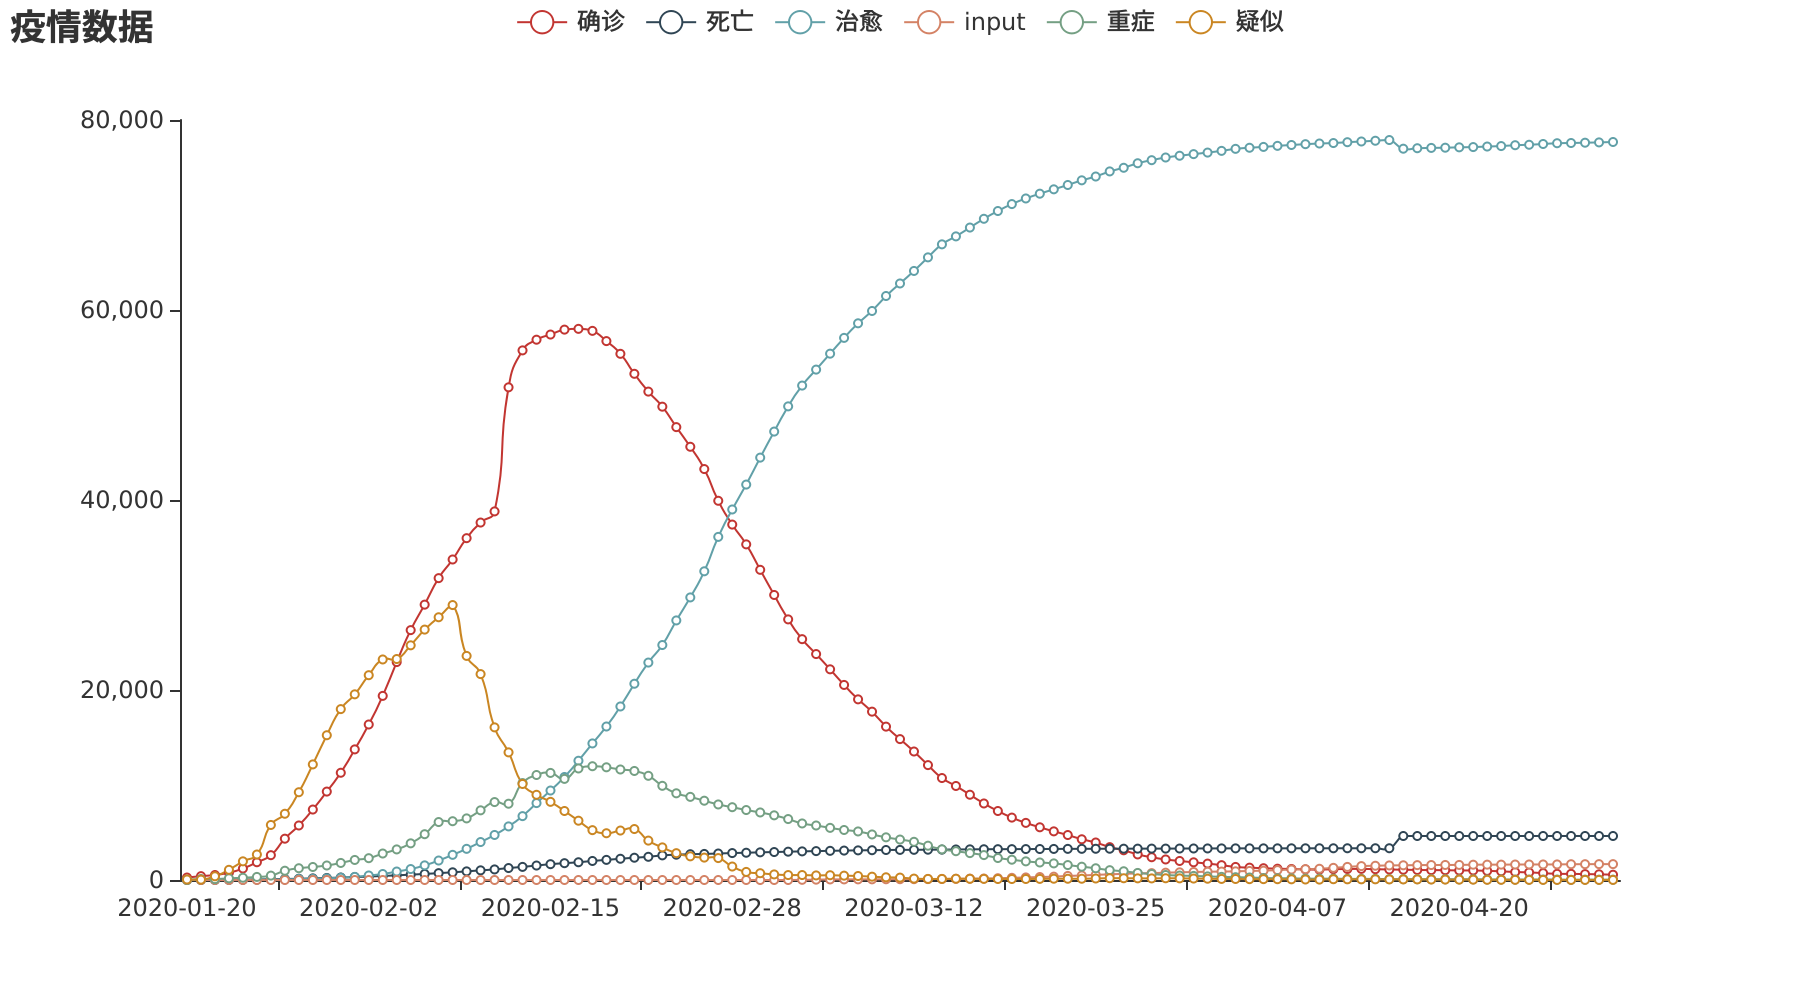
\includegraphics[width=\imagewidth]{疫情数据.png}
    \\
    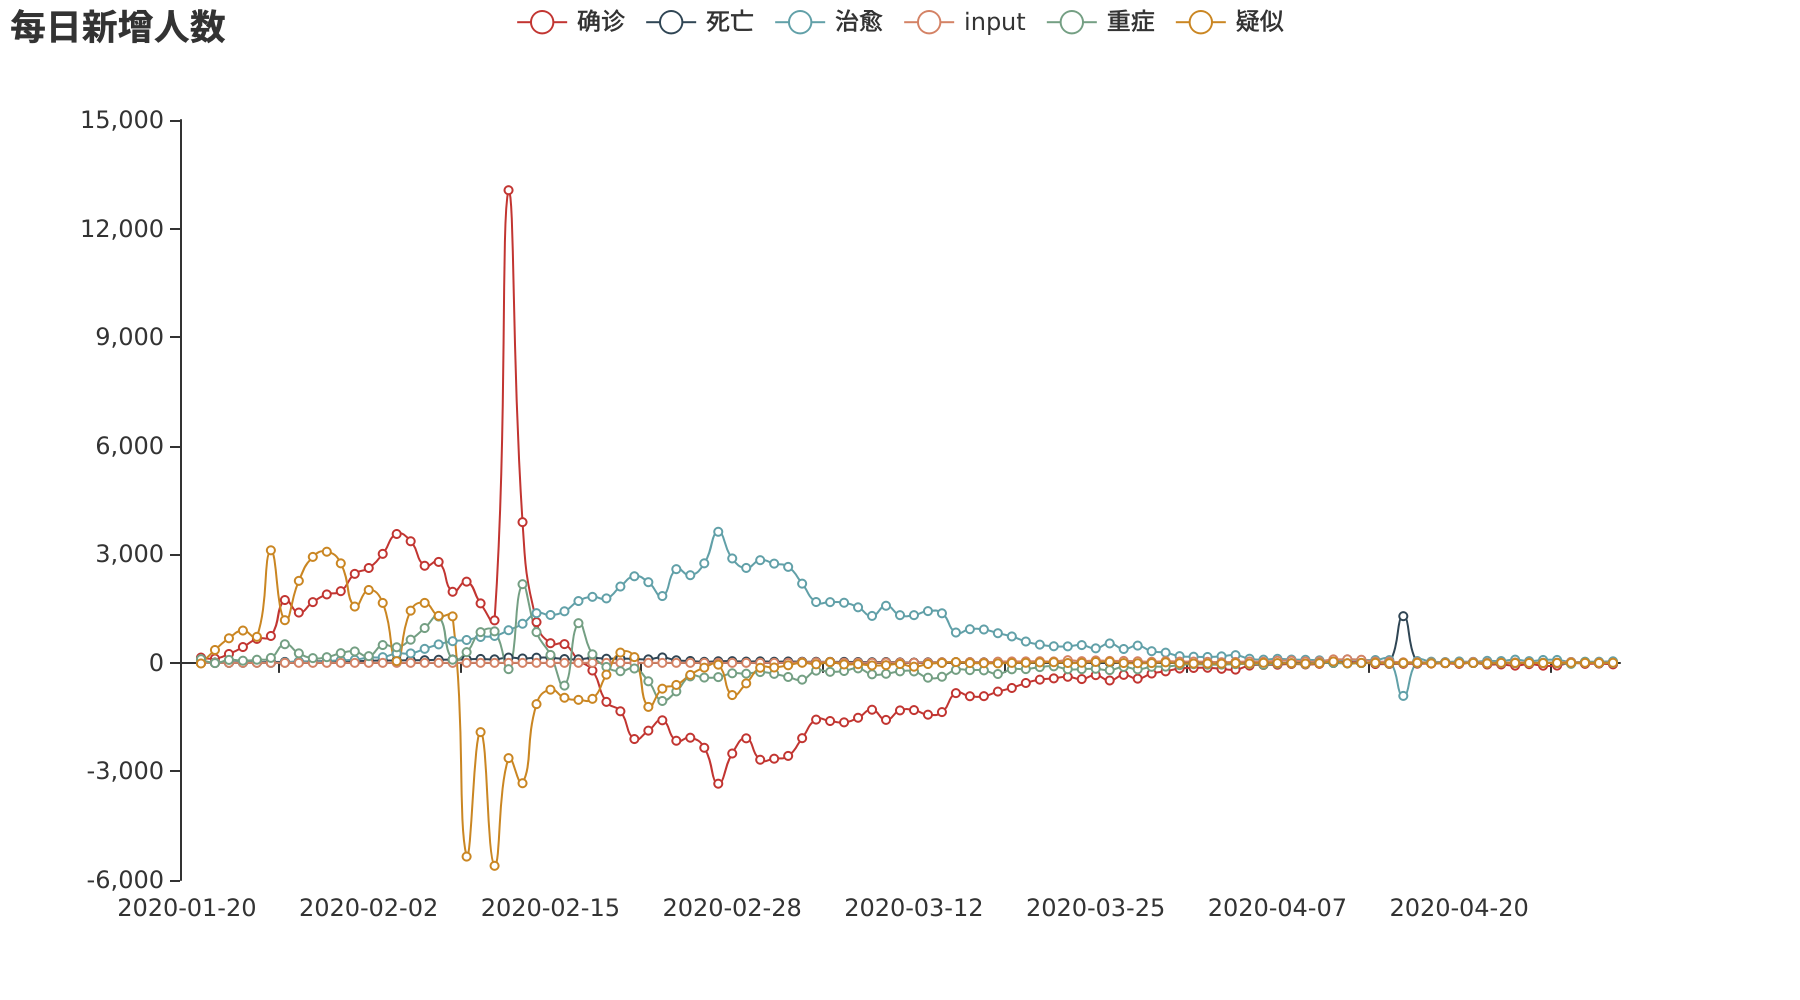
\includegraphics[width=\imagewidth]{每日新增人数.png}
    \par
    2月12日确诊人数猛增,
    是因为当日重新规定了确诊条件,
    导致许多疑似病例纳入确诊人数。
\end{appendix}
\end{document}